\documentclass[aspectratio=169]{beamer}
%\usepackage{svg}
\usepackage[american]{babel}

\usetheme[progressbar=frametitle,numbering=fraction,subsectionpage=progressbar]{metropolis}
\setbeamertemplate{section in toc}[sections numbered]
%\usepackage{appendixnumberbeamer}
\usepackage{ulem}
\usepackage[newfloat]{minted}
\usepackage{multicol}

\setminted[bash]{xleftmargin=\parindent,fontsize=\scriptsize,baselinestretch=1,breaklines, linenos}
\setminted[c++]{xleftmargin=\parindent,fontsize=\scriptsize,baselinestretch=1, breaklines,linenos}
\setminted[ruby]{xleftmargin=\parindent,fontsize=\scriptsize,baselinestretch=1, breaklines,linenos}
\setminted[fortran]{xleftmargin=\parindent,fontsize=\scriptsize,baselinestretch=1, breaklines,linenos}
\setminted[text]{xleftmargin=\parindent,fontsize=\scriptsize,baselinestretch=1}

\usepackage[export]{adjustbox}

\usepackage{tikz}
%\usetikzlibrary{positioning, matrix}
\usetikzlibrary{matrix, positioning, arrows.meta}
\usepackage{pgfplots}
\pgfplotsset{compat=1.18}

\setbeamertemplate{frame footer}{%
  
\includegraphics[height=0.5cm]{anl_logo_head.png}\hfill
  \texttt{extremecomputingtraining.anl.gov}}

\usepackage{booktabs}
\usepackage[autostyle, english=american]{csquotes}
\MakeOuterQuote{"}
\usepackage{caption}
\usepackage{subcaption}

\newcommand\blfootnote[1]{%
  \begingroup
  \renewcommand\thefootnote{}\footnote{#1}%
  \addtocounter{footnote}{-1}%
  \endgroup
}

\title{GPU Hardware Characteristics}
\subtitle{How does that even work? (ATPESC edition)}

\date{\today}
\author{Thomas Applencourt(apl@anl.gov)}
\titlegraphic{\hfill
\includegraphics[height=1.0cm,keepaspectratio]{anl_logo_head.png}}

% Argonne Color
\definecolor{mDarkTeal}{HTML}{000000}
\definecolor{mLightBrown}{HTML}{cb2332}
\definecolor{ANLBlue}{HTML}{1484c7}
\definecolor{ANLGreen}{HTML}{82c341}
\definecolor{ANLRed}{HTML}{CD202C}   % sampled from the red of the Argonne logo

\setbeamercolor{normal text2}{%
    fg=ANLRed,
    bg=black!2
}
\setbeamercolor{palette primary}{%
  use=normal text2,
  fg=normal text2.bg,
  bg=normal text2.fg
}
\setbeamercolor{frametitle}{%
  use=palette primary,
  parent=palette primary
}

\begin{document}

\maketitle

\begin{frame}{Outline}
\tableofcontents[hideallsubsections]
\end{frame}

\AtBeginSection[]{
  \begin{frame}{Outline}
    \tableofcontents[currentsection,hideothersubsections]
  \end{frame}
}


\begin{frame}{Who I'm ? (bias)}
\begin{itemize}
    \item Part of the Performance Enginiring Group (so we will discuss some tinming, and performance)
    \item Worked a lot, and for a long time, on Aurora (so we will use it sorry, and we will use Intel Hardware, but everything should (is?) transferable)
    \item Part of the SYCL Working-Group (so yeah, I like open stantard)
\end{itemize}
\end{frame}
% ===== MORNING: hardware characteristics =====
% ===================================================================
% MORNING TALK: "GPU Hardware Characteristics"
% Intro + What is a GPU? + Hands-on #1. (Unchanged content.)
% ===================================================================
\section{Introduction}

\begin{frame}{Key Question}
    \begin{itemize}
        \item What is the difference between a CPU and a GPU?
        \item Why we can use CUDA only on NVIDIA Hardware?
        \item Should I use OpenMP, SYCL or Kokkos? 
    \end{itemize}    
\end{frame}

\begin{frame}{Roadmap for my two sessions}
\begin{enumerate}
    \item \textbf{This morning --- What is a GPU?} Hardware in a nutshell:
          parallelism, the memory wall, the roofline. 
    \item \textbf{This afternoon --- Climbing the ladder}: from the low-level model
          up to SYCL / OpenMP / Kokkos, and why they are all the same idea.

\end{enumerate}

In between, the low-level ecosystem (CUDA / HIP / OpenCL).
\end{frame}

\section{What is a GPU?}                     

\begin{frame}{At the beginning was a loom\footnote{and then the Canuts, the Luddite, Engels' pause...}}

\begin{figure}
  \centering
  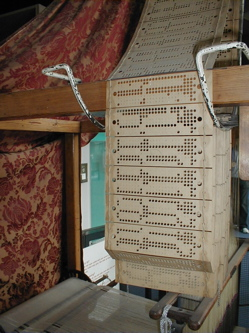
\includegraphics[width=0.27\linewidth]{Jacquard.loom.cards.jpg} 
  \caption{Late 1800s, Jacquard Machine: Threads and Warps}
\end{figure}


\end{frame}

\begin{frame}{NVIDIA in their wisdom reused some weaving terms}

\begin{figure}
    \centering
    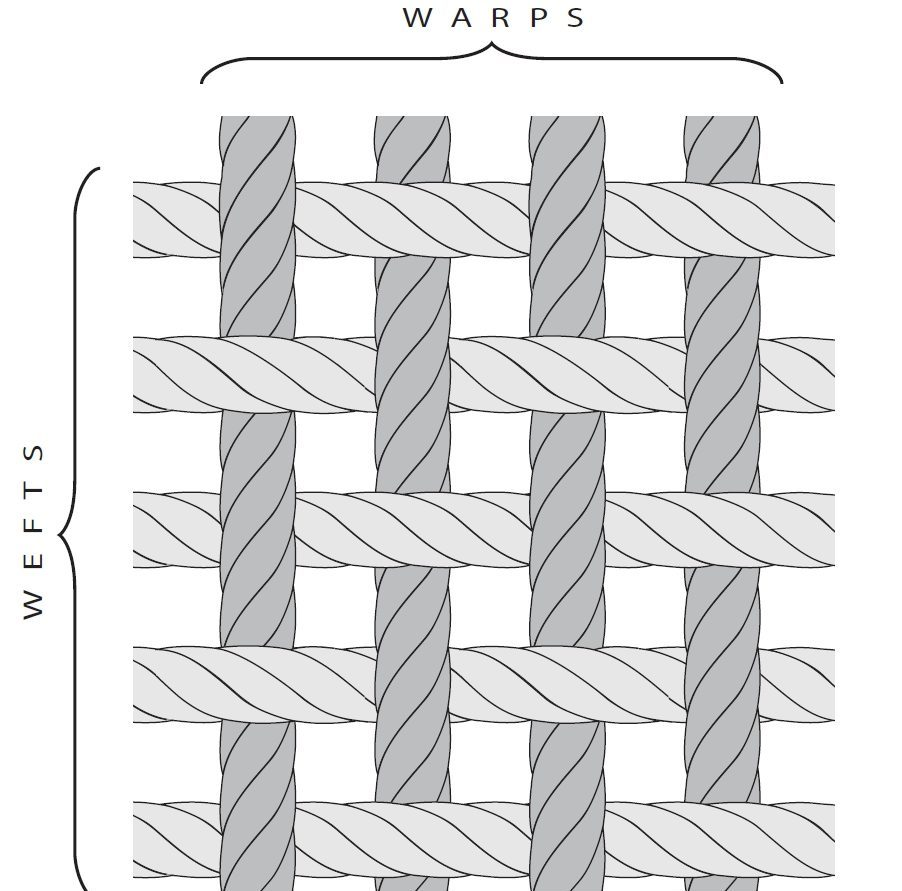
\includegraphics[width=0.30\linewidth]{wrap_thread.png}
    \caption{Warp and weft threads on a loom}
\end{figure}
Don't worry, later we will teach some less confusing terminology...
\end{frame}

\begin{frame}{And then CPU}

\begin{figure}
    \centering
    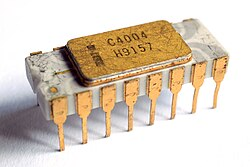
\includegraphics[width=0.5\linewidth]{image.png}
    \caption{ 1970, Intel 4004, 740 kHz, 2300 transistor}
\end{figure}

\end{frame}

\begin{frame}{How to get more performance?}
\begin{itemize}
    \item \textbf{Be Smarter} 
          \begin{itemize}
              \item Branch prediction\footnote{Speculative execution was a really good idea security wise...}, ILP (instruction level parallelism -- aka don't stall)
          \end{itemize}
    \item \textbf{Increase frequency!} Thread go faster!
          \begin{itemize}
            \item Core i9-14900K  (released in 2023) is 6 GHz
              \item One problem is power: $P \propto CV^2f$, and higher $f$ needs higher $V$ $\Rightarrow$ heat grows. 
              \item But still, still will not give you 2000x speed-up...
              
          \end{itemize}

    \item \textbf{What about doing more stuff in parallel?}
          \begin{itemize}
              \item SIMD (single instruction multiple data)
              \item More thread!
              \item This is Smart. We can always put "more" of stuff. "horizontal scaling"
          \end{itemize}
\end{itemize}

\end{frame}


\begin{frame}{Parallelism isn't new: vector computing is 50 years old}
\begin{columns}
\begin{column}{0.55\textwidth}
\begin{itemize}
    \item The \textbf{Cray-1} (1976) was a \textbf{vector} machine: one instruction
          over a whole vector of data.
    \item And then lots of CPUs work in parallel
    \item GPU is the same thing! \footnote{Kind of... with more limited synchronization}
\end{itemize}
\end{column}
\begin{column}{0.45\textwidth}
    \begin{figure}
    \centering
    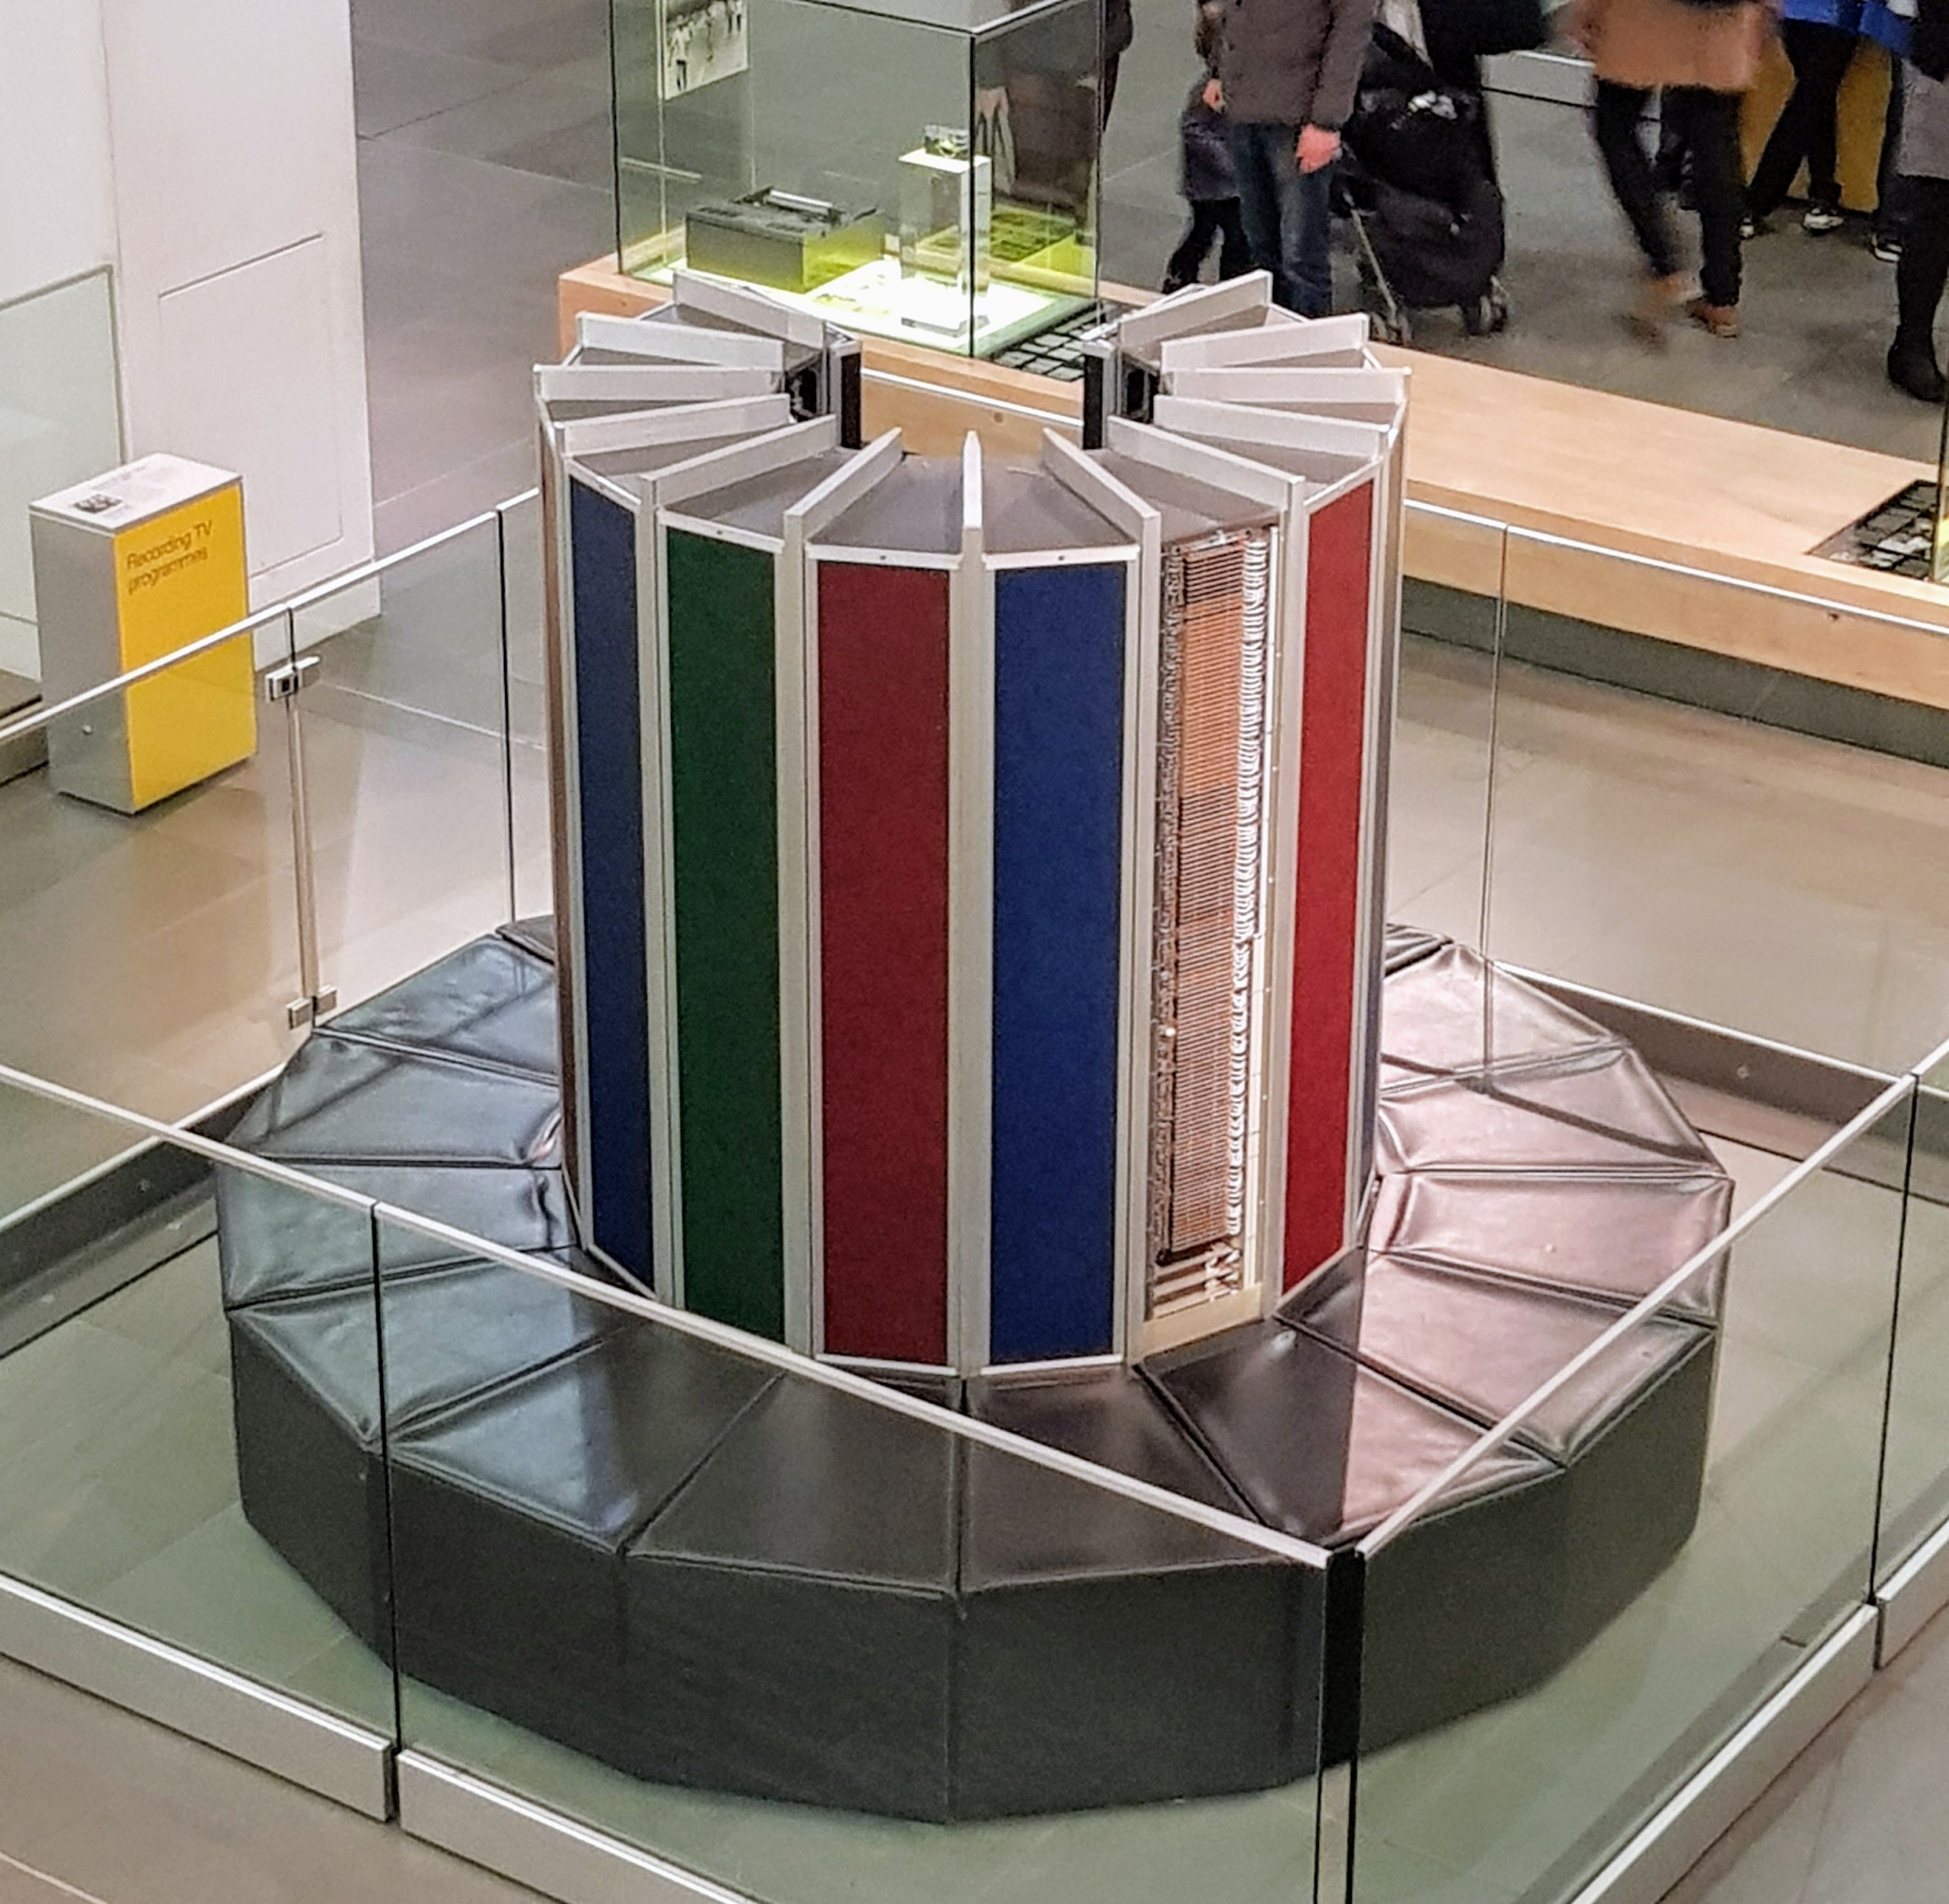
\includegraphics[height=0.7\textheight,keepaspectratio]{cray1.jpg}
    \caption{Cray-1, Science Museum London (CC BY-SA)}
    \end{figure}
\end{column}
\end{columns}

\end{frame}


\begin{frame}{And then come GPU...}

Let's just put more parallelism. No sync between them. Just for "embarrassingly-parallel" applications. Like... drawing pixels on a screen? Graphics Processing Unit
\end{frame}

\begin{frame}{It's just}


\begin{itemize}
    \item A GPU $\approx$ a very "stupid" CPU with a huge number of wide SIMD threads.
    \item And then people realised that GPU can be used to do some Linear Algebra. So why not... GP-GPU General-Purpose Graphics Processing Unit (means nothing already...)
    \item CPU followed a similar pattern, just added more threads, but smart threads. (All those ooo) and fancy synchronization (software threads can "time-slice / hyper-threading"), they can be stopped, and restarted (preemption).
\end{itemize}

And the lines are blurring: Top500 \#1 is a \textbf{pure-CPU} machine with 304
cores per socket\footnote{LineShine, Shenzhen (Top500, June 2026).}
\end{frame}




\begin{frame}{Some Terminology}

\begin{center}
\begin{tabular}{@{}ll@{}}
\toprule
\textbf{SIMD lane}        & Work on one data element \\
\textbf{SIMD instruction} & Work on multiple data at once \\
\textbf{Hardware thread}  & Execute a list of SIMD Instructions \\
\bottomrule
\end{tabular}
\end{center}

\begin{itemize}
    \item Each Hardware Thread runs some \textbf{SIMD instructions}
    \item For example Intel PVC GPU has 3{,}584 hardware threads concurrently on 512 bits wide data \footnote{Pro tips: All the HW have some register to know "where" you are running in the hardware. Not super public, but not secret either: \texttt{HW\_REG\_HW\_ID2} for AMD and \texttt{intel\_get\_slice\_id} for example}
\end{itemize}

\end{frame}

\begin{frame}{One instruction, many lanes}
\begin{center}
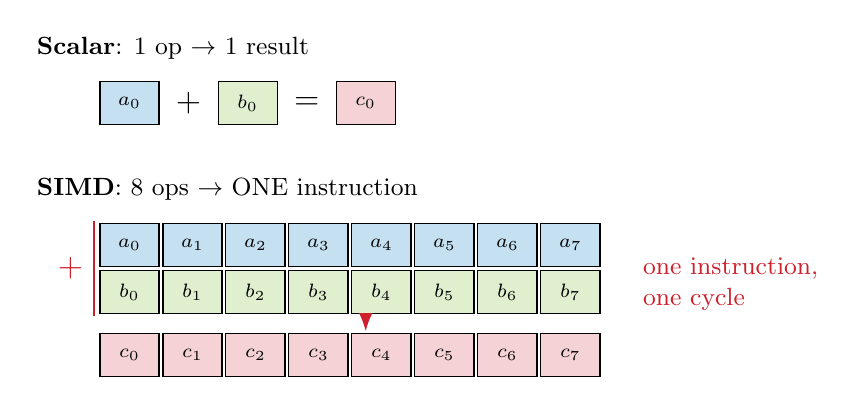
\begin{tikzpicture}[
    font=\scriptsize,
    lane/.style={draw, minimum width=0.75cm, minimum height=0.55cm},
    op/.style={font=\large}
]
% ---------- Scalar ----------
\node[anchor=west, font=\small] at (-1.3,2.9) {\textbf{Scalar}: 1 op $\rightarrow$ 1 result};
\node[lane, fill=ANLBlue!25]  at (0.0,2.2) {$a_0$};
\node[op] at (0.75,2.2) {$+$};
\node[lane, fill=ANLGreen!25] at (1.5,2.2) {$b_0$};
\node[op] at (2.25,2.2) {$=$};
\node[lane, fill=ANLRed!20]   at (3.0,2.2) {$c_0$};

% ---------- SIMD ----------
\node[anchor=west, font=\small] at (-1.3,1.1) {\textbf{SIMD}: 8 ops $\rightarrow$ \alert{ONE} instruction};
\foreach \i in {0,...,7} {
    \node[lane, fill=ANLBlue!25]  at (\i*0.8, 0.4) {$a_{\i}$};
    \node[lane, fill=ANLGreen!25] at (\i*0.8,-0.2) {$b_{\i}$};
    \node[lane, fill=ANLRed!20]   at (\i*0.8,-1.0) {$c_{\i}$};
}
% single-instruction annotation spanning all lanes
\draw[ANLRed, thick] (-0.45,0.7) -- (-0.45,-0.5);
\node[op, ANLRed] at (-0.75,0.1) {$+$};
\draw[-{Latex}, ANLRed, thick] (3.0,-0.5) -- (3.0,-0.7);
\node[anchor=west, ANLRed, font=\small, align=left] at (6.4,-0.1) {one instruction,\\ one cycle};
\end{tikzpicture}
\end{center}

\begin{itemize}
    \item Same opcode, same cycle --- the \textbf{lane count is the SIMD width} (here 8; PVC is 16 floats wide).
    \item A \textbf{hardware thread} just streams a list of these wide instructions.
\end{itemize}
\end{frame}

\begin{frame}{How do you get so many hardware threads? Replication (same as HPC)}

\begin{figure}
    \centering
    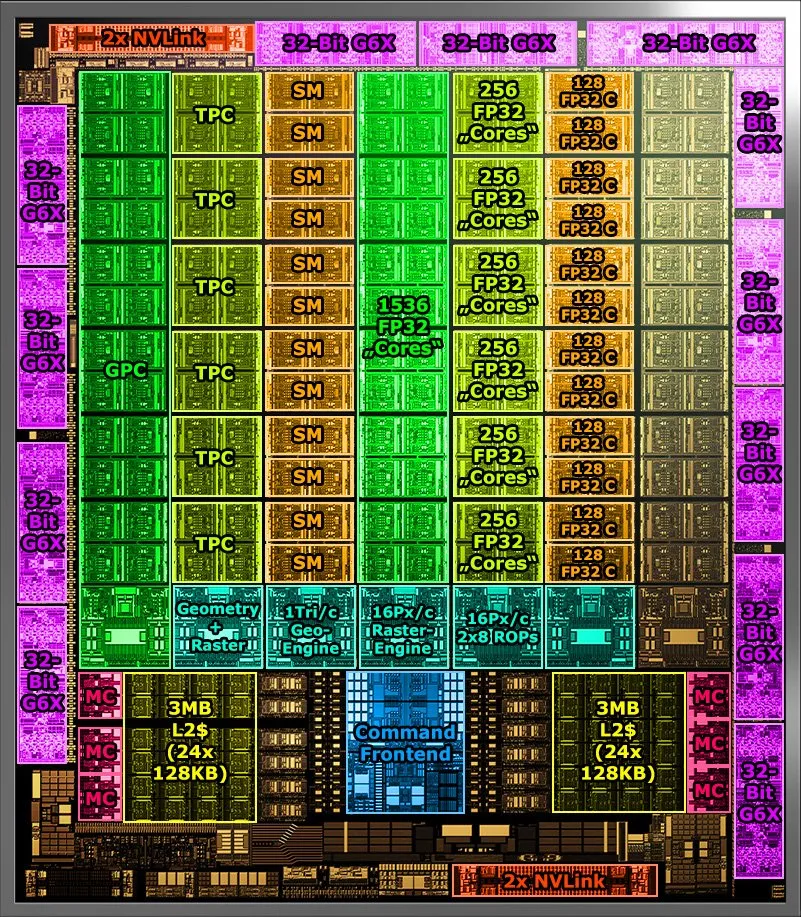
\includegraphics[width=0.40\textwidth,keepaspectratio]{locuza_ga102.png}
    \caption{Annotated NVIDIA GA102 die. Image credit: Locuza}
\end{figure}


\end{frame}

\begin{frame}{PVC Slice Example (not a real picture)}

\begin{figure}
    \centering
    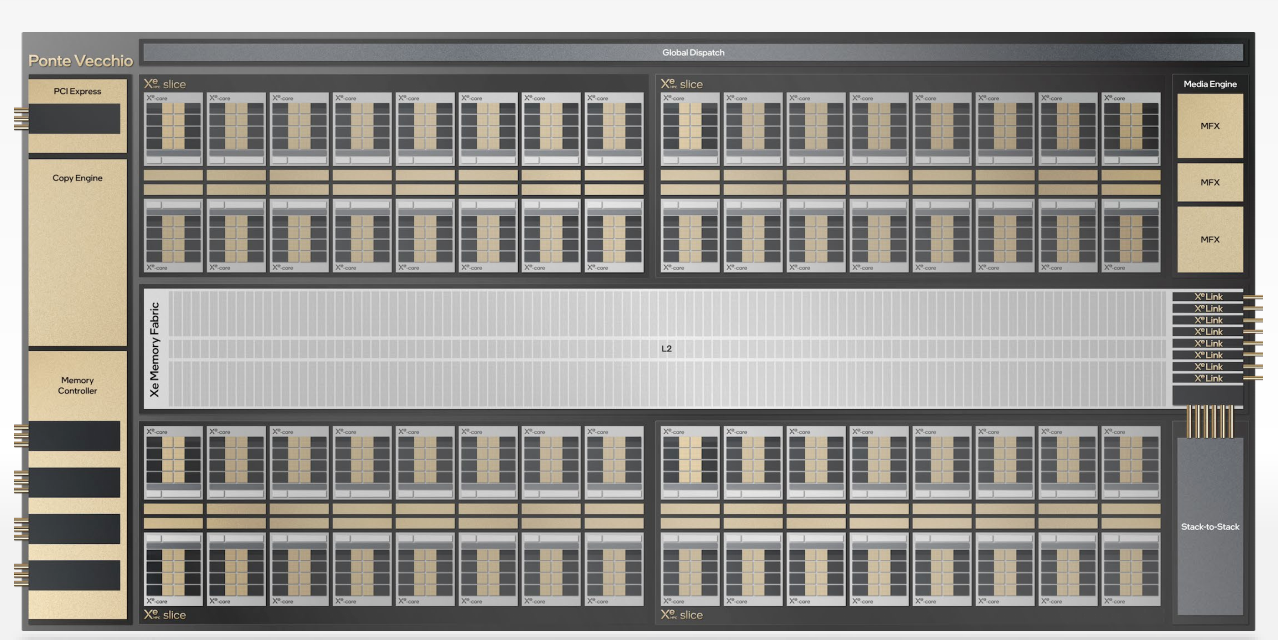
\includegraphics[width=1.0\linewidth]{pvc_slice.png}
\end{figure}
\end{frame}

\begin{frame}{Terminology}

No, I really don't want to talk about different vendors naming things differently for fun.
It's not fun.

Just some stuff share a L1, then an L2, and then nothing.  And then they are interconnected.
That's it (SM, Slice, GCD, whatever, doesn't matter. What matters is the topology)
\end{frame}

\begin{frame}{Let's still try...}

\begin{figure}
    \centering
    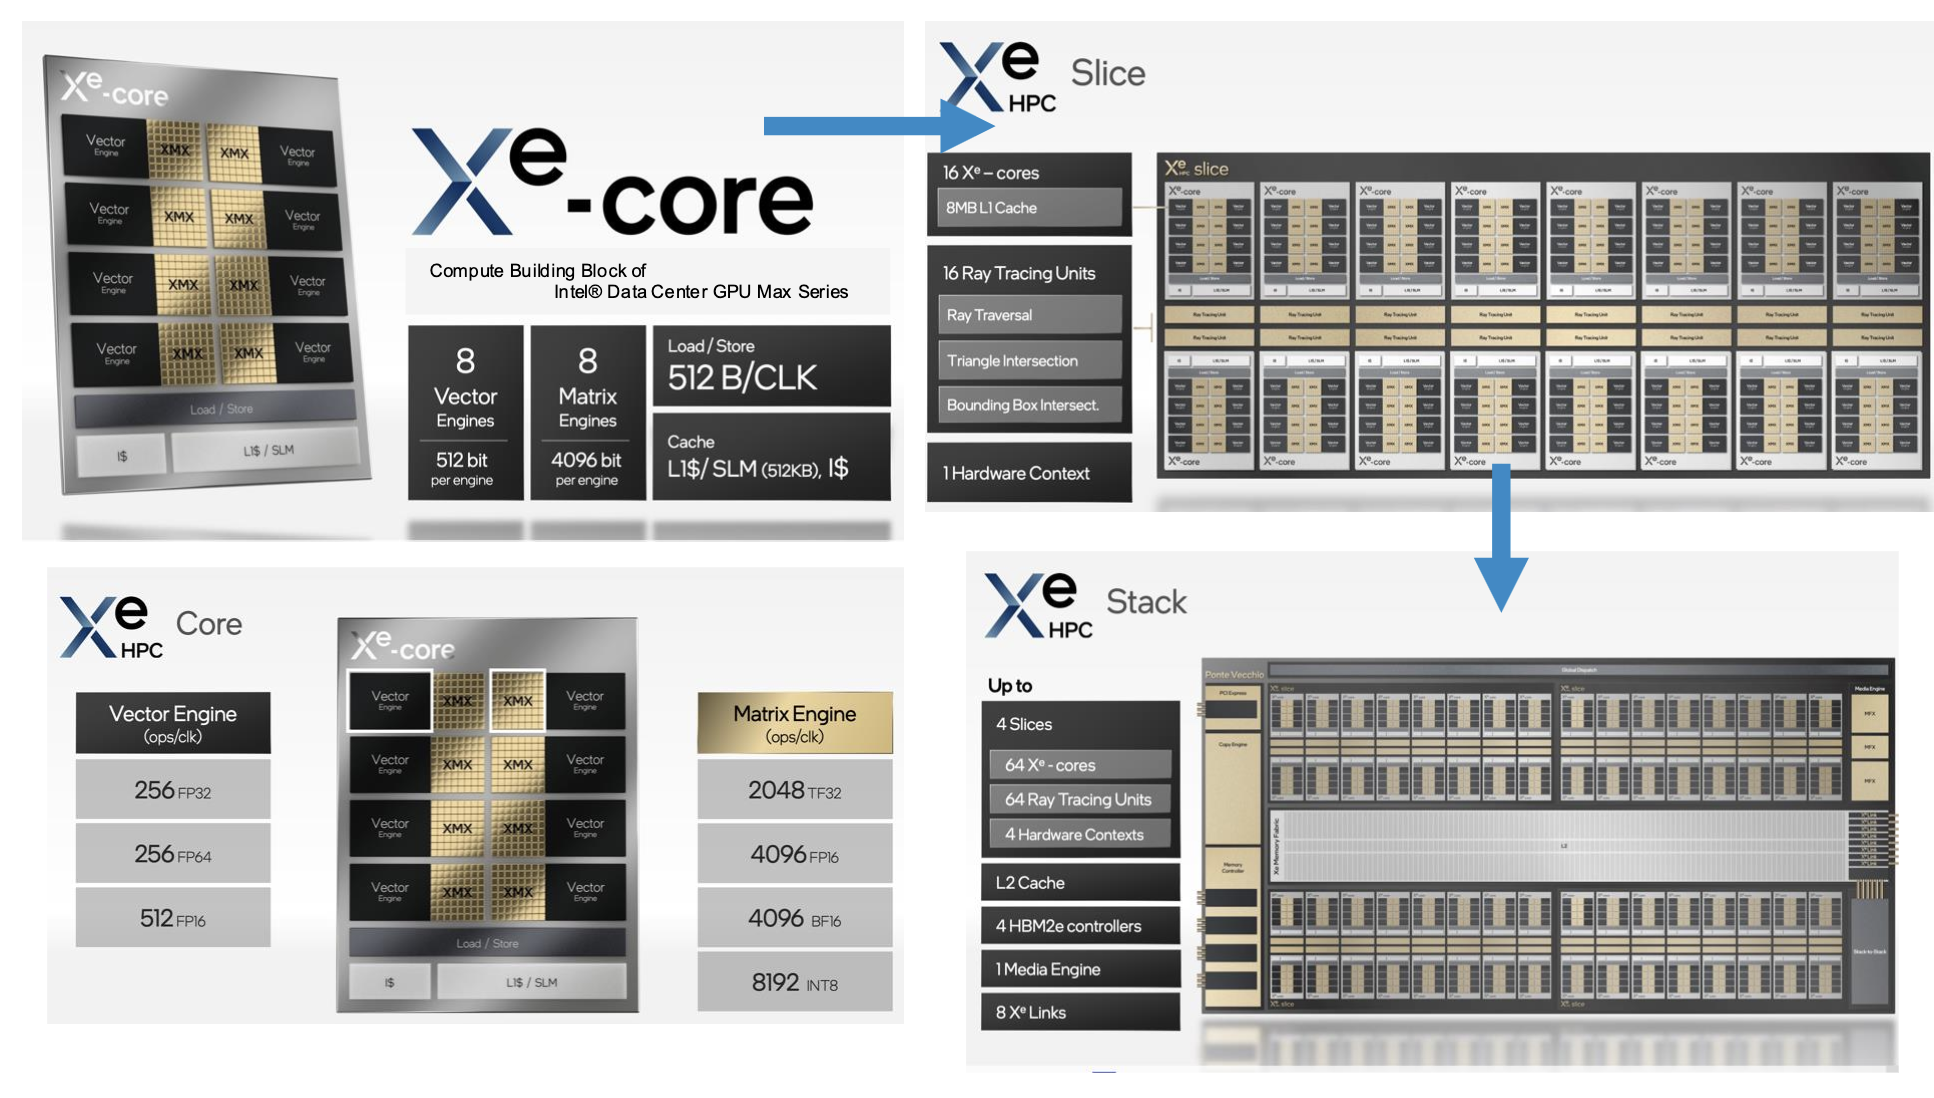
\includegraphics[width=0.8\linewidth]{intel_terminology.png}
    \caption{Intel Terminology}
\end{figure}

\end{frame}

\begin{frame}{I prefer the "logical" view}

\begin{itemize}
    \item Forget the names. What matters: \textbf{what do they share}, and
          \textbf{can they synchronize}?
    \item \textbf{Inside one Xe Core}: shared L1 / shared-local-memory, and lanes
          \alert{can sync} --- this is the compute unit (the SM / CU equivalent).
    \item \textbf{Across Xe Cores / tiles}: only an L2, then the interconnect ---
          \alert{no sync}. Same story on every vendor.
\end{itemize}

\end{frame}

\begin{frame}{Same thing, three vendors' names}

\begin{center}
\begin{tabular}{@{}llll@{}}
\toprule
\textbf{Concept} & \textbf{NVIDIA} & \textbf{AMD} & \textbf{Intel} \\
\midrule
SIMD group (lanes lock-step) & warp (32) & wavefront (64) & SIMD8/16/32 \\
\alert{Compute unit} (shares L1, \alert{can sync}) & SM & CU & Xe Core \\
Fast local memory            & shared mem & LDS & SLM \\
Whole die / tile (\alert{no sync across}) & GPU & GCD & Xe Stack \\
\bottomrule
\end{tabular}
\end{center}
\medskip
\begin{itemize}
    \item The \alert{sync boundary} is the row that matters: inside the compute
          unit you can sync + share fast memory; above it you cannot.
    \item Everything else is marketing.
\end{itemize}
\end{frame}
% === NEW  (the key restriction: no sync across hardware threads)
\begin{frame}{The one big restriction: limited synchronization}
\begin{itemize}
    \item Inside \textbf{one hardware thread}: lanes can
          sync\footnote{Obviously as most of the time they executed a lock-step}. 
    \item Across \textbf{hardware threads} running on the same core: you can sync, and have access to some fast "shared-local-memory" aka "Managed L1 cache"
    \item Between cores, it's not ok. No SYNC. There is no "global synchronization" on GPU. \footnote{I mean you can always be non-portable and do so. But threads are not "preemptable" so they cannot hit the barrier, and "make room" for other threads. They are not, because then it's not a GPU, it's a CPU. And it would be too complex / expensive, submission overhead would be huge, etc etc. Trade-off overhead}
\end{itemize}
\end{frame}

\begin{frame}{Why that restriction is a gift}
Because the hardware threads are independent, the scheduler is trivial:
\begin{itemize}
    \item If the HW has nothing to execute, just take some work.
    \item A HW thread is never \textbf{preempted} --- its registers stay live for
          its whole lifetime, so a context switch costs nothing (there is nothing
          to save/restore).
    \item So  when one HW stalls (on memory for example), another runs. That is
          how \alert{latency is hidden}, for free.
\end{itemize}
\alert{The restriction (no global sync) is exactly what buys the parallelism.}
Freedom vs.\ performance --- the GPU takes performance. Fast to schedule.
\end{frame}

\begin{frame}{Recap}
    \begin{itemize}
        \item Lots of Threads running Concurrently
        \item Not that much synchronization possible
        \item The hard thing is not really programming the GPU, it's designing an algorithm that is "embarrassingly-parallel"
        \item But at the bottom of it, this is what HPC is all about: Extracting concurrency from your algorithm/problem
    \end{itemize}
\end{frame}

% #####################################################################
\section{Performance --- Hands-on \#1}
% #####################################################################

\begin{frame}{Let's talk about performance}
Before we get started, just in case:
\begin{itemize}
    \item \textbf{FLOP} = one floating-point operation (a count). One FMA
          $a{=}b{\cdot}c{+}d$ is \textbf{2 FLOP} (but one instruction). \textbf{FLOP/S}, is FLOP per Second\footnote{and don't use FLOPS... just confusing. And I will make this mistake many times, sorry.}
\end{itemize}

We will assess the Peak FP32 of your favorite Hardware: One tile of PVC
\end{frame}

\begin{frame}{Just need to have some data}

\begin{itemize}
    \item  how many HW Threads we have,
    \item  The size of the SIMD instruction (aka how many FLOP they can do in 1 instruction)
    \item And the Frequency
    \item Then just multiply
\end{itemize}

\end{frame}

\begin{frame}[fragile]{Step 1 --- ask the hardware (\texttt{ze\_info})}
\begin{itemize}
    \item Get a node
    \item Then run \mintinline{bash}{ZE_AFFINITY_MASK=0.0 ze_info}
    \item ...
    \item  Profit (give me a number on slack). The people who have it correctly (and can explain) win a sticker!
\end{itemize}

\end{frame}
% --- Beat 1, step 1: ask the hardware
\begin{frame}[fragile]{Step 1 --- ask the hardware (\texttt{ze\_info}): Solution}
One tile (\texttt{ZE\_AFFINITY\_MASK=0.0}):
\begin{minted}{text}
Core Clock Rate             1500MHz
Physical EU SIMD Width      16      # FP32 lanes (8 for FP64)
Number EU Per SubSlice      8       # vector engines / Xe-Core
Number SubSlices Per Slice  56      # Xe-Cores per tile
Number Slices               1       # one tile
\end{minted}

Yeah, enjoy different terminology. Fun isn't it?
\end{frame}

\begin{frame}{Step 2 --- derive the theoretical peak}
Nothing magic --- just multiply the fields (FP32, one tile):
\medskip
\begin{center}
\small
$\underbrace{16}_{\substack{\text{SIMD width}\\ \text{(FP32 lanes)}}}
 \times \underbrace{8}_{\substack{\text{vector eng.}\\ \text{/ Xe-Core}}}
 \times \underbrace{56}_{\text{Xe-Cores}}
 \times \underbrace{2}_{\text{FMA}}
 \times \underbrace{1.5}_{\text{GHz}}
 \;=\; \mathbf{21{,}504}\ \text{GFLOP/s}$
\end{center}

Next question: How much of this we can reach? Any guess?
\end{frame}

\begin{frame}{Step 3 --- measure it}

\begin{itemize}
    \item I give you 3 binaries, each to measure one key characteristic.
    \item By default they use one HW thread, you can pass as argument the number you want
    \item  Enjoy compiling it. It's always one of the most fun parts...
\end{itemize}

How much? With how many HW threads used?

\medskip

Extra credit (a gift): can you write one kernel that reaches
\textbf{both} the compute and bandwidth peak at once? If somebody can do it, win a 1 dollar Cray Coin!

\end{frame}


% --- Beat 1, step 3: measure it
\begin{frame}{Step 3 --- measure all three roofs}
Run the three provided benchmarks; compare to what the hardware promised:
\begin{center}
\begin{tabular}{@{}llr@{}}
\toprule
\textbf{Benchmark} & \textbf{Roof} & \textbf{Measured} \\
\midrule
\texttt{flops} & compute (21{,}504 theo.) & \alert{21{,}427 GFLOP/s} ($\sim$99.6\%) \\
\texttt{triad} & HBM bandwidth            & \alert{$\sim$1{,}000 GB/s} \\
\texttt{pci}   & host $\leftrightarrow$ device (PCIe) & \alert{$\sim$75 GB/s} \\
\bottomrule
\end{tabular}
\end{center}
\medskip
\begin{itemize}
    \item  99\% for HBM. Easy!
    \item \textbf{Feel the gap}: HBM is $\sim$10--100$\times$ slower than compute,
          PCIe another $\sim$10--100$\times$ below HBM.
    \item  So yeah, compute fast, data-transfer slow.

\end{itemize}
\end{frame}

% === Beat 2: the FLOPs are not the bottleneck --- the memory wall
\begin{frame}{Memory wall: data movement, not FLOPs}
\begin{itemize}
    \item Compute is cheap, \textbf{data movement is expensive}: the bottleneck is
          almost always memory, not FLOPs.
    \item \textbf{Discrete GPU}: separate memory, so you must ship data over PCIe.
          Slow --- minimize transfers, keep data resident, recompute over reload.
\end{itemize}
\end{frame}

\begin{frame}{Side story: discrete accelerator $\rightarrow$ integrated}
The same cycle plays out every time, e.g.\ the floating-point unit:
\begin{itemize}
    \item \textbf{Discrete first.} The x87 math coprocessor was a separate chip
          you socketed: 8087 (with 8086/8088), 80287 (286), 80387 (386).
    \item \textbf{Then integrated.} The 486DX (1989) put the FPU on the CPU die.
          Nobody thinks of "the FPU" as a separate thing anymore.
\end{itemize}
\alert{GPUs are following the exact same path}: discrete PCIe cards today
$\rightarrow$ integrated tomorrow (APUs, MI300A, Grace-Hopper\ldots).

No silver bullet. Now we have NUMA effects. Maybe better than PCIe but not "free" either.
Locality is, always will be, key for Performance
\end{frame}


% === NEW  (arithmetic intensity: compute- vs memory-bound)
\begin{frame}{Arithmetic intensity: flop per byte}
\textbf{Arithmetic intensity} = FLOP done $/$ bytes moved. It decides whether you
are compute- or memory-bound. 

\end{frame}

% === NEW  (the money slide: the roofline, with all three roofs, measured PVC)
\begin{frame}{The roofline (one PVC tile, Single Precision)}
\begin{center}
\begin{tikzpicture}
\begin{loglogaxis}[
    width=0.82\textwidth, height=0.66\textheight,
    xlabel={arithmetic intensity (flop/byte)},
    ylabel={GFLOP/s},
    xmin=0.1, xmax=10000, ymin=10, ymax=100000,
    xtick={0.1,1,10,100,1000,10000},
    ytick={10,100,1000,10000,100000},
    tick label style={font=\scriptsize}, label style={font=\scriptsize},
    legend style={font=\scriptsize, at={(0.02,0.98)}, anchor=north west,
                  draw=none, fill=white, fill opacity=0.7, text opacity=1},
    grid=both, major grid style={black!12},
]
% Compute roof: 21427 GFLOP/s (flat)
\addplot[very thick, mDarkTeal, domain=0.1:10000, samples=2] {21427};
\addlegendentry{compute roof (21{,}427)}
% HBM roof: y = 1000 * AI, capped at compute roof (ridge at AI=21.4)
\addplot[very thick, ANLBlue] coordinates {(0.1,100) (21.4,21427) (10000,21427)};
\addlegendentry{HBM roof (1{,}000 GB/s)}
% PCIe roof: y = 75 * AI (ridge at AI=286)
\addplot[very thick, mLightBrown] coordinates {(0.133,10) (286,21427) (10000,21427)};
\addlegendentry{PCIe roof (75 GB/s)}
% Workload dots
\addplot[only marks, mark=*, mark size=2.5pt, black] coordinates {(0.17,167)};
\node[font=\scriptsize, anchor=west] at (axis cs:0.21,167) {triad (BW-bound)};
\addplot[only marks, mark=*, mark size=2.5pt, black] coordinates {(8000,21427)};
\node[font=\scriptsize, anchor=south east] at (axis cs:7000,21427) {FMA chain (compute-bound)};
% The ridge: the ONE point touching both roofs -- the extra-credit target
\addplot[only marks, mark=star, mark size=4pt, ANLGreen, very thick] coordinates {(21.4,21427)};
\node[font=\scriptsize\bfseries, ANLGreen, anchor=north west] at (axis cs:25,19000) {can you reach this?};
\end{loglogaxis}
\end{tikzpicture}
\end{center}
\vspace{-0.5em}
Below AI $\approx$20 you are HBM memory-bound; below $\sim$286 you are PCIe-bound.

\end{frame}

\begin{frame}{Just to be super clear}

AI is per byte. So for each byte you read from main memory you need to do at least 20 FLOP:
\begin{itemize}
    \item so you need at least 80 FLOP per float!  Enjoy being compute bound guys.
    \item And you have at least 7168 simd-lanes to use. If you use less, you are not fully utilizing the full compute capability of one Tile.
    \item Oh, and we have 63744 GPUs on Aurora, so you just need to use 913\_833\_984 vector lines every cycle \footnote{So if your "problem space" is lower than that, it's mathematically impossible to use Aurora at max capacity}
\end{itemize}


\end{frame}

\begin{frame}{Conclusion: GPU in a nutshell}
\begin{itemize}
    \item A wide-SIMD, latency-hiding throughput machine.
    \item The naming does matter, it's just hierarchical. You have some levels where sync is free, some where it's expensive, some where it's impossible.
    \item Fast because it is simple: no big caches, no branch prediction,
          no fancy per-lane cleverness.
    \item Gap between Memory and Flops is huge. You need to compute, compute, compute
    \item GPUs are big. And we have many of them. So please extract the maximum concurrency of your simulation. And avoid reading from main memory\footnote{cache -> data locality, re-computing}
\end{itemize}

\end{frame}

\begin{frame}{Thanks!}

I think we have a Q\&A now. 
\end{frame}



% ===== AFTERNOON: second title slide =====
\title{Higher Level Layer: SYCL/OpenMP/Kokkos}
\subtitle{How does that even work? (ATPESC edition)}
\maketitle

% ===== AFTERNOON: higher-level programming models =====
% =====================================================================
% AFTERNOON TALK: "Higher Level Layer: SYCL / OpenMP / Kokkos"
% Draft of the new \section{Climbing the Ladder} + Hands-on #2.
% Story arc (4 acts): the hard way -> not magic (thomas) -> same idea /
% 3 models / standards -> performance (async vs blocking, ordering).
% All code snippets below were compiled + run on PVC (Max 1550), L2=0.
% =====================================================================

\section{Higher Level: Climbing the Ladder}

\begin{frame}{Before we start: some terminology so we speak the same language}
    \begin{itemize}
        \item Work-Item, Sub-Group, Work-group
    \end{itemize}
\end{frame}

\usetikzlibrary{fit,backgrounds,calc}
\begin{frame}{Now we can name it: the software hierarchy}
Same picture as the hardware sync boundary --- this time in \textbf{SYCL} words.
Each \textbf{work-item} runs its own stream of instructions (top arrows).
\begin{center}
\begin{tikzpicture}[font=\scriptsize, >=Stealth,
  wi/.style={rectangle, draw=ANLBlue!70, fill=ANLBlue!15,
             minimum width=5.5mm, minimum height=5.5mm, inner sep=1pt},
  sg/.style={draw=ANLGreen!75!black, fill=ANLGreen!18, rounded corners,
             inner sep=2.6mm, line width=1pt},
  wg/.style={draw=ANLRed!80, fill=ANLRed!6, rounded corners,
             inner sep=4mm, line width=1pt},
  instr/.style={->, black!55, line width=0.5pt, shorten >=0.4mm}]

  % ===== Work-group 0 : two sub-groups of four work-items =====
  \node[wi]                     (a11) {};
  \node[wi, right=1.1mm of a11] (a12) {};
  \node[wi, right=1.1mm of a12] (a13) {};
  \node[wi, right=1.1mm of a13] (a14) {};
  \node[wi, below=9mm of a11]   (a21) {};
  \node[wi, right=1.1mm of a21] (a22) {};
  \node[wi, right=1.1mm of a22] (a23) {};
  \node[wi, right=1.1mm of a23] (a24) {};

  % ===== Work-group 1 =====
  \node[wi, right=50mm of a14]  (b11) {};
  \node[wi, right=1.1mm of b11] (b12) {};
  \node[wi, right=1.1mm of b12] (b13) {};
  \node[wi, right=1.1mm of b13] (b14) {};
  \node[wi, below=9mm of b11]   (b21) {};
  \node[wi, right=1.1mm of b21] (b22) {};
  \node[wi, right=1.1mm of b22] (b23) {};
  \node[wi, right=1.1mm of b23] (b24) {};

  % ===== Ghost work-group (0..N): invisible anchors midway between A and B =====
  \node[wi, draw=none, fill=none] (g11) at ($(a11)!0.5!(b11)$) {};
  \node[wi, draw=none, fill=none, right=1.1mm of g11] (g12) {};
  \node[wi, draw=none, fill=none, right=1.1mm of g12] (g13) {};
  \node[wi, draw=none, fill=none, right=1.1mm of g13] (g14) {};
  \node[wi, draw=none, fill=none] (g21) at ($(a21)!0.5!(b21)$) {};
  \node[wi, draw=none, fill=none, right=1.1mm of g21] (g22) {};
  \node[wi, draw=none, fill=none, right=1.1mm of g22] (g23) {};
  \node[wi, draw=none, fill=none, right=1.1mm of g23] (g24) {};

  % ---- boxes: work-group FIRST, then sub-groups on top (so green shows) ----
  \begin{scope}[on background layer]
    % ghost work-group behind, faded + dashed
    \node[wg, dashed, draw=ANLRed!40, fill=ANLRed!3, fit=(g11)(g24)] (wgG) {};
    \node[sg, dashed, draw=ANLGreen!45!black!60, fill=ANLGreen!8, fit=(g11)(g14)] {};
    \node[sg, dashed, draw=ANLGreen!45!black!60, fill=ANLGreen!8, fit=(g21)(g24)] {};
    % solid work-groups
    \node[wg, fit=(a11)(a24)] (wgA) {};
    \node[wg, fit=(b11)(b24)] (wgB) {};
    \node[sg, fit=(a11)(a14)] (sgA1) {};
    \node[sg, fit=(a21)(a24)] (sgA2) {};
    \node[sg, fit=(b11)(b14)] (sgB1) {};
    \node[sg, fit=(b21)(b24)] (sgB2) {};
  \end{scope}

  % ---- instruction stream: a little arrow above every work-item ----
  \foreach \n in {a11,a12,a13,a14,a21,a22,a23,a24,b11,b12,b13,b14,b21,b22,b23,b24}{
    \draw[instr] ($(\n.north)+(0,4mm)$) -- ($(\n.north)+(0,0.6mm)$);
  }
  \node[font=\scriptsize\itshape, text=black!60, anchor=south]
    at ($(a12.north)!0.5!(a13.north)+(0,4.5mm)$) {instructions};

  % ---- work-group labels (below) ----
  \node[anchor=north, yshift=-0.5mm] at (wgA.south) {\textbf{Work-group 0}};
  \node[anchor=north, yshift=-0.5mm] at (wgB.south) {\textbf{Work-group N}};

  % ===== "no sync" dividers flanking the ghost work-group =====
  \draw[ANLRed, dashed, line width=0.9pt]
    ($(wgA.north east)!0.5!(wgG.north west)$) --
    ($(wgA.south east)!0.5!(wgG.south west)$);
  \draw[ANLRed, dashed, line width=0.9pt]
    ($(wgG.north east)!0.5!(wgB.north west)$) --
    ($(wgG.south east)!0.5!(wgB.south west)$);
  \node[ANLRed, align=center, font=\scriptsize\bfseries, fill=black!2, inner sep=1pt]
    at ($(wgA.east)!0.5!(wgG.west)$) {NO\\sync};
  \node[ANLRed, align=center, font=\scriptsize\bfseries, fill=black!2, inner sep=1pt]
    at ($(wgG.east)!0.5!(wgB.west)$) {NO\\sync};
  % ellipsis over the ghost = "work-groups 0 .. N"
  \node[font=\Large\bfseries, text=black!35] at (wgG.center) {$\cdots$};
\end{tikzpicture}
\end{center}

\begin{center}\scriptsize
\tikz[baseline=-0.6ex]\node[draw=ANLBlue!70, fill=ANLBlue!15, minimum size=3mm, inner sep=0pt]{};\,\textbf{work-item} (SIMD lane)\quad
\tikz[baseline=-0.6ex]\node[draw=ANLGreen!75!black, fill=ANLGreen!18, rounded corners, minimum size=3mm, inner sep=0pt]{};\,\textbf{sub-group}\quad
\tikz[baseline=-0.6ex]\node[draw=ANLRed!80, fill=ANLRed!6, rounded corners, minimum size=3mm, inner sep=0pt]{};\,\textbf{work-group}
\end{center}
\end{frame}

\begin{frame}{Now we can name it: the software hierarchy}
\begin{itemize}
  \item \textbf{Work-item} inside a \textbf{sub-group}: sync is fast, lanes share
        registers (\texttt{shuffle} / cross-lane ops).
  \item \textbf{Sub-group} inside a \textbf{work-group}: share \alert{Shared Local Memory}
        (SLM), can \texttt{barrier()}.
  \item Between \textbf{work-groups}: \alert{no synchronization possible} --- they are
        independent, may not even be co-resident.
  \item The model only guarantees \textbf{forward progress within one work-group}
        (conceptually "one at a time"). The \alert{hardware} may run many at once ---
        but you cannot rely on it.
\end{itemize}
\end{frame}

\begin{frame}{Recap to previous session (hopefully)}
\begin{itemize}
    \item A \textbf{host program}, with a C API driving it: find device, load the binary, make a queue, allocate memory, copy, launch kernel, synchronize.
    \item The kernel is written into a separate file.
\end{itemize}
This afternoon: the same thing, but with syntactic sugar\footnote{And we have enough diabetes... Please don't make your own candy factory}
\end{frame}



\begin{frame}[fragile]{[One C API to] in the darkness bind them}

create/load/launch dance:
\begin{minted}{c++}
// Intel / OpenCL                       // NVIDIA / CUDA Driver
clCreateProgramWithIL(spirv,...);    |   cuModuleLoad(&m, "hello.ptx");
clCreateKernel(prog,"saxpy");        |   cuModuleGetFunction(&f,m,"saxpy");
clSetKernelArg(...); ...             |   cuLaunchKernel(f, grid, block, ...);
clEnqueueNDRangeKernel(q,k,...);      
\end{minted}
\begin{itemize}
    \item  I will not discuss the `<<</>>>` cuda syntax. \footnote{It's not valid C. You need a special compiler pass to parse that... Thanks NVIDIA}
    \item Explicit, just a C compiler and ... \textbf{tedious}.
    \item Every high-level programming model is "this, wrapped." Nothing more.
    \item Layers, layers everywhere
\end{itemize}

\end{frame}



\begin{frame}{Talking about higher-level programming models\footnote{"Where is my Vulkan?" Sorry gamer people... OpenCL $\to$ Vulkan exists. Rusticl!}}

\begin{center}
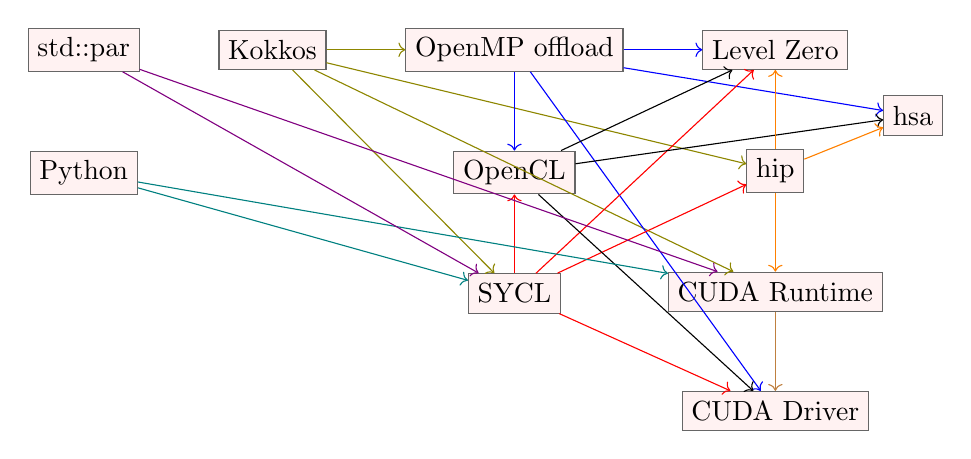
\begin{tikzpicture}[
nnode/.style={rectangle, draw=black!60, fill=red!5, minimum size=5mm},
]

\node[nnode]      (kokkos)                      {Kokkos};
\node[nnode]      (omp)      [right=of kokkos]  {OpenMP offload};
\node[nnode]      (stdpar)   [left=of kokkos]   {std::par};
\node[nnode]      (py)       [below=of stdpar]  {Python};
\node[nnode]      (opencl)   [below= of omp]     {OpenCL};
\node[nnode]      (sycl)     [below=of opencl]     {SYCL};

\node[nnode]      (ze)       [right=of omp]    {Level Zero};

\node[nnode]      (hip)      [below=of ze]      {hip};
\node[nnode]      (hsa)      [yshift=2em, right=of hip]     {hsa};

\node[nnode]      (cr)       [below=of hip]     {CUDA Runtime};
\node[nnode]      (cd)       [below=of cr]     {CUDA Driver};

\draw[->,draw=olive] (kokkos) -- (omp);
\draw[->,draw=olive] (kokkos) -- (sycl);
\draw[->,draw=olive] (kokkos) -- (hip);
\draw[->,draw=olive] (kokkos) -- (cr);

\draw[->,draw=blue] (omp) -- (opencl);
\draw[->,draw=blue] (omp) -- (hsa);
\draw[->,draw=blue] (omp) -- (cd);
\draw[->,draw=blue] (omp) -- (ze);


\draw[->,draw=red] (sycl) -- (opencl);
\draw[->,draw=red] (sycl) -- (ze);
\draw[->,draw=red] (sycl) -- (hip);
\draw[->,draw=red] (sycl) -- (cd);

\draw[->] (opencl) -- (cd);
\draw[->] (opencl) -- (ze);
\draw[->] (opencl) -- (hsa);

\draw[->, draw=orange] (hip) -- (ze);
\draw[->, draw=orange] (hip) -- (cr);
\draw[->, draw=orange] (hip) -- (hsa);

\draw[->,draw=brown] (cr) -- (cd);

% Python: mostly wraps SYCL (dpnp/dpctl) and CUDA (CuPy/PyTorch)
\draw[->,draw=teal] (py) -- (sycl);
\draw[->,draw=teal] (py) -- (cr);

% std::par: SYCL on Intel, CUDA on NVIDIA (nvc++ -stdpar)
\draw[->,draw=violet] (stdpar) -- (sycl);
\draw[->,draw=violet] (stdpar) -- (cr);

\end{tikzpicture}
\end{center}
\end{frame}



\begin{frame}{Note on compilation: two compilers}
\begin{center}
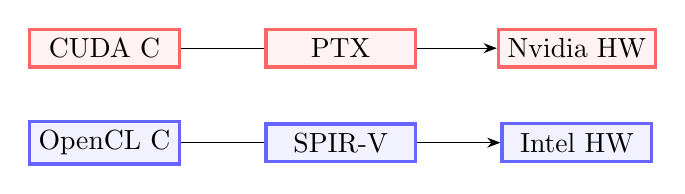
\begin{tikzpicture}[
    x=3.0cm, y=1.2cm, >=Stealth,
    nnode/.style={rectangle, draw=red!60,  fill=red!5,  very thick, minimum width=1.9cm, align=center},
    anode/.style={rectangle, draw=green!60,fill=green!5,very thick, minimum width=1.9cm, align=center},
    inode/.style={rectangle, draw=blue!60, fill=blue!5, very thick, minimum width=1.9cm, align=center},
  ]
  \node[nnode] (cudac)   at (0,0)  {CUDA~C};
  \node[nnode] (ptx)     at (1,0)  {PTX};
  \node[nnode] (Nvidiah) at (2,0)  {Nvidia HW};
  \node[inode] (openclc) at (0,-1) {OpenCL~C};
  \node[inode] (spirv)   at (1,-1) {SPIR-V};
  \node[inode] (intelh)  at (2,-1) {Intel HW};
  \draw[->] (cudac) -- (ptx)  -- (Nvidiah);
  \draw[->] (openclc) -- (spirv) -- (intelh);
\end{tikzpicture}
\end{center}
\begin{itemize}
    \item You can generate PTX, or SPIR-V, from multiple "source languages"
    \item Rust, Fortran, Python, whatever.
\end{itemize}
\end{frame}

% ------------------------------------------------------------------
% ACT 2 --- Not magic: single source + build your own tiny layer
% ------------------------------------------------------------------
\begin{frame}[fragile]{Single-source: let's build our own. It's not magic}

Let's build a 40-line version of this. Your own little single-source, higher-level language!\footnote{Please don't do that at home, just for illustration purposes, to remove the magic. It's not magic, just painful to maintain}

\begin{itemize}
    \item Tell the compiler what is a kernel
    \item It will generate the SPIR-V for you
    \item Wrap everything in a tiny runtime
\end{itemize}
Let me introduce you to \textsc{Thomas}:
\begin{itemize}
    \item \textbf{T}iny --- \textbf{H}eterogeneous --- \textbf{O}penCL ---
          \textbf{M}acro --- \textbf{A}TPESC --- \textbf{S}PIR-V
\end{itemize}
\end{frame}

\begin{frame}[fragile]{Single-source: let's build our own --- \textsc{Thomas}}


Our own little single-source wrapper.\footnote{\textsc{Thomas}: \textbf{T}iny
\textbf{H}eterogeneous \textbf{O}penCL \textbf{M}acro, \textbf{A}TPESC +
\textbf{S}PIR-V.}
\begin{minted}{c++}
#include "thomas.hpp"
KERNEL(triad, (float a, gptr<const float> x, gptr<const float> y, gptr<float> z),
       { z[i] = x[i] + a*y[i]; })
int main() {
  thomas::init();                          // pick the GPU
  float *x = thomas::alloc<float>(N);      // USM: one pointer, host + device
  float *y = thomas::alloc<float>(N), *z = thomas::alloc<float>(N);
  for (size_t i = 0; i < N; ++i) { x[i] = 2.0f; y[i] = 1.0f; }
  thomas::parallel_for(N, triad, 2.0f, x, y, z);   // bind args, launch on GPU
}
\end{minted}
\end{frame}

\begin{frame}[fragile]{How it works: one source, compiled twice}
The \emph{same} file is compiled twice --- the \texttt{KERNEL} macro expands
differently each time:
\begin{itemize}
    \item \textbf{Device pass}: \mintinline{bash}{icpx -x cl -cl-std=clc++ -DTHOMAS_DEVICE}
          turns the lambda into a \texttt{\_\_kernel} and lowers it to SPIR-V.
    \item \textbf{Host pass}: plain \mintinline{bash}{icpx} keeps only the kernel
          \emph{name}, embeds the SPIR-V, and drives OpenCL.
    \item \texttt{gptr<T>} is \texttt{\_\_global T*} on the device, plain
          \texttt{T*} on the host --- one signature, both passes.
\end{itemize}
\begin{minted}{c++}
// DEVICE pass -- lambda body becomes a __kernel
#define KERNEL(name, params, body) \
  __kernel void name params { auto _k=[&](ulong i) body; _k(get_global_id(0)); }

// HOST pass -- keep only the name to find the compiled kernel
#define KERNEL(name, params, body) ::thomas::Kernel name{#name};
\end{minted}
\end{frame}



\begin{frame}[fragile]{Not magic (2/2): the whole "runtime" is a few calls}
The device pass emits SPIR-V; the host side just loads it and launches. That is the
entire "runtime":
\begin{minted}{c++}
// load our compiled SPIR-V and JIT it for whatever device we picked
prog = clCreateProgramWithIL(ctx, thomas_spv, thomas_spv_len, &e);
clBuildProgram(prog, 1, &dev, ...);
// parallel_for: bind args, launch N work-items
clSetKernelArg(...);  clEnqueueNDRangeKernel(q, k, 1, 0, &N, ...);
\end{minted}
Built twice (device$\rightarrow$SPIR-V, host), the triad ran on one PVC tile ---
right on top of SYCL, because it \emph{is} the same thing (resident USM + SPIR-V):
\begin{minted}{text}
THOMAS    N=1048576  min_ms=0.013  BW=960 GB/s  residual=0
SYCL      N=1048576  min_ms=0.013  BW=960 GB/s  residual=0
\end{minted}
\alert{$\sim$40 lines over OpenCL + SPIR-V. That is all SYCL/Kokkos are, plus a lot of bug fixes, syntactic sugar, and runtime optimization}
\end{frame}


\begin{frame}{I will now show you some programming models}

Comparative literature!

I will show you
\begin{itemize}
    \item SYCL (the best)
    \item Kokkos (the best)
    \item OpenMP (the best)
    \item  std-par (the best)
    \item Python\footnote{not the best, sorry, I'm just old. Using a scripting language for HPC just seems wrong. I don't like Jupyter notebooks either, so this one is maybe on me}
\end{itemize}

\end{frame}


\begin{frame}{The models, one by one}
The next few slides: who backs each model, what it looks like, and what it runs
on. Same kernel everywhere --- only the packaging changes.
\begin{center}\small
\begin{tabular}{@{}lll@{}}
\toprule
Model & Kind & Backed by \\
\midrule
\textbf{SYCL}       & open standard, pure C++      & Khronos \\
\textbf{Kokkos}     & C++ portability library      & Sandia / HPSF \\
\textbf{OpenMP}     & directive (pragma) standard  & OpenMP ARB \\
\texttt{std::par}   & ISO C++ standard library     & ISO C++ \\
\textbf{Python}     & array libraries / bindings   & vendors \\
\bottomrule
\end{tabular}
\end{center}
\end{frame}

% ---- SYCL ------------------------------------------------------------
\begin{frame}{SYCL --- the open C++ standard}
\begin{itemize}
  \item Backed by \textbf{Khronos}\footnote{The OpenCL / Vulkan / SPIR-V people.}
        --- an open standard, not one vendor's product.
  \item \textbf{Pure C++}: a light abstraction over the native backend, with full
        control when you want it.
  \item Two main implementations:
    \begin{itemize}
      \item \textbf{Intel oneAPI DPC++} --- \href{https://github.com/intel/llvm}{github.com/intel/llvm}
      \item \textbf{AdaptiveCpp} (higher-level, ex-hipSYCL) ---
            \href{https://github.com/AdaptiveCpp/AdaptiveCpp}{github.com/AdaptiveCpp/AdaptiveCpp}
    \end{itemize}
  \item Backends: \textbf{CUDA, OpenCL, Level~Zero, FPGA}.
\end{itemize}
\vfill
{\footnotesize Spec \& overview: \href{https://www.khronos.org/sycl/}{khronos.org/sycl}}
\end{frame}

% ---- Kokkos ----------------------------------------------------------
\begin{frame}{Kokkos --- the C++ portability library}
\begin{itemize}
  \item Developed at \textbf{Sandia National Laboratories}; now governed by the
        \textbf{High Performance Software Foundation} (part of the Linux Foundation).
  \item \textbf{C++} with a portability abstraction on top (\texttt{View},
        execution/memory spaces).
  \item Ships as a \textbf{library} --- super easy to install (\texttt{module load}
        or CMake).
  \item Backends: \textbf{SYCL, CUDA, HIP}, and an \textbf{OpenMP host} backend.
\end{itemize}
\vfill
{\footnotesize Home \& docs: \href{https://kokkos.org}{kokkos.org}}
\end{frame}

% ---- OpenMP ----------------------------------------------------------
\begin{frame}{OpenMP --- directives (pragmas)}
\begin{itemize}
  \item \textbf{Pragma-based}: you annotate a loop, the compiler offloads it ---
        no library API to learn.
  \item Works from \textbf{C, C++, and Fortran}\footnote{Sad face? Happy face? I
        let you decide.} --- the only model here that covers Fortran.
  \item Descriptive: you still write the loop; the pragma says "run this on the
        device."
\end{itemize}
\vfill
{\footnotesize Spec: \href{https://www.openmp.org}{openmp.org}}
\end{frame}

% ---- std::par --------------------------------------------------------
\begin{frame}{\texttt{std::par} --- it's just ISO C++}
\begin{itemize}
  \item \textbf{No pragma, no library}: parallel algorithms are in the C++
        standard itself (C++17).
  \item Pass an \textbf{execution policy} (\texttt{std::execution::par\_unseq})
        to \texttt{std::for\_each}, \texttt{transform}, \ldots
  \item The compiler/runtime decides where it runs --- on Intel, that's the GPU.
\end{itemize}
\vfill
{\footnotesize Reference:
\href{https://en.cppreference.com/w/cpp/algorithm/execution_policy_tag}{cppreference: execution policies}}
\end{frame}

% ---- Python ----------------------------------------------------------
\begin{frame}{Python --- multiple GPU array bindings}
\begin{itemize}
  \item Not one thing: several \textbf{NumPy-style array libraries} that run on the GPU.
  \item \textbf{dpnp} (Intel, SYCL/Level~Zero) ---
        \href{https://github.com/IntelPython/dpnp}{github.com/IntelPython/dpnp}
  \item \textbf{CuPy} (NVIDIA/AMD) ---
        \href{https://cupy.dev}{cupy.dev}
  \item Same \texttt{a*x + y} you'd write in NumPy --- it just lands in a GPU kernel.
\end{itemize}
\end{frame}

\begin{frame}[fragile]{Same kernel, three models --- C++ (all run on PVC)}
\begin{columns}[T]
\begin{column}{0.5\textwidth}
\textbf{SYCL} \footnotesize(Khronos standard)
\begin{minted}{c++}
sycl::queue Q;
auto x = malloc_shared<float>(N,Q); 
auto y = malloc_shared<float>(N,Q); 
Q.parallel_for(N, [=](auto i){
  y[i] = a*x[i] + y[i];
}).wait();
\end{minted}
\textbf{Kokkos} \footnotesize(portability library)
\begin{minted}{c++}
Kokkos::View<float*> x("x",N), y("y",N);
Kokkos::parallel_for(N,
  KOKKOS_LAMBDA(size_t i){
    y(i) = a*x(i) + y(i);
});
Kokkos::fence();   // async; sync to time/read
\end{minted}
\end{column}
\begin{column}{0.5\textwidth}
\textbf{OpenMP target} \footnotesize(directives)
\begin{minted}{c++}
#pragma omp target teams \
  distribute parallel for \
  map(to:x[0:N]) map(tofrom:y[0:N])
for (int i=0;i<N;i++)      // explicit
  y[i] = a*x[i] + y[i];    // loop!
\end{minted}
\alert{Squint --- they are the same kernel.}
Same index space, same lambda body, same
$y = a x + y$.
\end{column}
\end{columns}
\end{frame}

\begin{frame}[fragile]{Same kernel, higher still --- standard languages \& Python}
\begin{columns}[T]
\begin{column}{0.52\textwidth}
\textbf{C++ \texttt{std::par}} \footnotesize(ISO C++, no pragma)
\begin{minted}{c++}
std::for_each(std::execution::par_unseq,
  idx.begin(), idx.end(),
  [=](size_t i){ y[i]=a*x[i]+y[i]; });
\end{minted}
\textbf{Fortran \texttt{do concurrent}} \footnotesize(ISO Fortran)
\begin{minted}{fortran}
do concurrent (i = 1:N)
   y(i) = a*x(i) + y(i)
end do
\end{minted}
\end{column}
\begin{column}{0.48\textwidth}
\textbf{Python (dpnp)}
\begin{minted}{python}
import dpnp
x = dpnp.ones(N, dtype=dpnp.float32)
y = dpnp.full(N, 2.0, dtype=dpnp.float32)
y = a*x + y          # runs on the GPU
\end{minted}
\footnotesize

\end{column}
\end{columns}
\end{frame}

\begin{frame}{Some difference}
\begin{center}
\begin{tabular}{@{}llll@{}}
\toprule
 & Kernel is & Data & Default submit \\
\midrule
SYCL           & lambda (C++)    & USM pointers / buffers   & \textbf{async} \\
Kokkos         & lambda (C++)    & \texttt{View} + spaces   & \textbf{async} \\
OpenMP         & \textbf{explicit loop} & \texttt{map} clauses & \textbf{blocking} \\
\texttt{std::par} & lambda (C++) & normal containers        & \textbf{blocking} \\
\bottomrule
\end{tabular}
\end{center}
{\footnotesize OpenMP \texttt{target} is blocking by default; add \texttt{nowait}+\texttt{depend} for async.}
{\footnotesize SYCL's default queue is the only \textbf{out-of-order} one; the rest are effectively in-order.}

\begin{itemize}
    \item \textbf{OpenMP is descriptive}: you write the loop, the pragma offloads it.
          The others hide the loop inside \texttt{parallel\_for}.
    \item \textbf{Async default} (SYCL/Kokkos) vs \textbf{blocking default} (OpenMP)
          --- this drives performance (we come back to it in Act~4).
\end{itemize}
\end{frame}

\begin{frame}{Where does the data live? Three styles}
The kernel is only half the story --- you also decide how memory moves.
\begin{enumerate}
    \item \textbf{Raw pointer, explicit.} You allocate on the device and copy
          yourself. SYCL USM, OpenMP 6 allocation, our \textsc{thomas}.
          Most control, most boilerplate.
    \item \textbf{OpenMP \texttt{map} clauses.} \texttt{map(to:/from:/tofrom:)} ---
          the runtime tracks what is already present and moves the rest. Depends on
          the surrounding \texttt{target data} region.
    \item \textbf{Implicit objects.} \texttt{sycl::buffer}\footnote{We will not talk about those, nobody uses those}, Kokkos \texttt{View} /
          \texttt{DualView}, the object owns the data and the runtime moves it
          where a kernel needs it.
\end{enumerate}

\end{frame}

\begin{frame}{One pointer, three flavors}

\begin{center}
\begin{tabular}{@{}ll p{4.9cm}@{}}
\toprule
Khronos\footnote{In Khronos land we call all three \textbf{Unified Shared Memory} (USM); it just means ``pointer access.'' \texttt{shared} and \texttt{host} are a subset of USM} & CUDA / HIP & What it means \\
\midrule
device memory & device memory  & only accessible by the \textbf{device} \\
shared memory & managed memory & accessible by \textbf{host and device}; data may migrate between them \\
host memory   & pinned memory  & accessible by \textbf{both}; data stays on the host (can speed up transfers) \\
\bottomrule
\end{tabular}
\end{center}


\end{frame}

\begin{frame}[fragile]{Kokkos adds data abstractions: \texttt{View} \& \texttt{DualView}}
SYCL/OpenMP move data with pointers. Kokkos provides some abstractions:

\begin{minted}{c++}
Kokkos::View<float*, MemSpace> d("d", N);   // layout + space chosen for the arch
Kokkos::DualView<float*> v("v", N);         // a host mirror AND a device copy
v.modify_device();                          // lazy H2D: just marks dirty, 0 bytes
v.sync_host();                              // sync, copy if required
\end{minted}
\begin{itemize}
    \item \texttt{View}: memory \textbf{space} (host/device) + \textbf{layout}
          (row/col-major) picked per architecture --- portability of data, not
          just kernels.
    \item \texttt{DualView}: manage the host$\leftrightarrow$device copy explicitly,
          only sync when a side is dirty. (USM hides this; Kokkos gives you control.)
    \item Some of these abstractions were \textbf{upstreamed into the C++ standard} ---
          e.g.\ \texttt{std::mdspan} (C++23). It's super nice.
\end{itemize}
\end{frame}

\begin{frame}[fragile]{\texttt{std::mdspan}: a Kokkos \texttt{View} that made it into C++23}
A non-owning, multi-dimensional \textbf{view} over a flat buffer --- index it like
\texttt{a(i,j)}, no manual \texttt{i*ncols+j}:
\begin{minted}{c++}
#include <mdspan>
float buf[6];                                 // plain, flat storage
std::mdspan a{buf, 2, 3};                      // view it as 2 x 3

for (std::size_t i = 0; i < a.extent(0); ++i)  // extent(0)=2, extent(1)=3
  for (std::size_t j = 0; j < a.extent(1); ++j)
    a[i, j] = i * 10 + j;                       // C++23 multidim subscript
\end{minted}
\begin{itemize}
    \item Owns \textbf{nothing} --- just shape + a pointer. Same idea as Kokkos
          \texttt{View}, now standard.
    \item Swap the \textbf{layout} (row- vs column-major) without touching the loop ---
          exactly the portability trick Kokkos does per architecture.
    \item \textbf{Fortran} has had native N-D arrays since day one (1957); C++ only
          gets the \emph{view} now, in 2023.\footnote{Better late than never.}
\end{itemize}
\end{frame}

\begin{frame}[fragile]{Lambda vs pragma: what the compiler has to know}
Everyone here needs a device compiler (our \textsc{thomas} used one too:
\texttt{-x cl -cl-std=clc++}). The real split is \textbf{how the kernel is
represented}.
\begin{itemize}
    \item \textbf{SYCL / Kokkos / \texttt{std::par}: the kernel is a lambda} --- a
          plain C++ object the library can capture, store and pass to
          \mintinline{c++}{parallel_for}. So the layer above is ordinary library
          code (AdaptiveCpp even has a library-only path). \alert{The \texttt{parallel\_for}
          we wrote in \textsc{thomas} is exactly that.}
    \item \textbf{OpenMP / \texttt{do concurrent}: the kernel is a pragma / language
          construct.} \mintinline{c++}{#pragma omp target} is not a C++ object --- a
          library cannot see it. The \textbf{compiler} must recognize it and emit the
          device code.
\end{itemize}
\alert{Both need a toolchain to reach the device. A lambda is a value you can hand
around; a pragma only the compiler can act on.}
\end{frame}



\begin{frame}{Let's run!}

\begin{itemize}
    \item I prepared a few code examples that do the triad
    \item Let's run them. And let's see who is faster
    \item And let's discuss their differences, similarities. Answer any question
\end{itemize}

\end{frame}


\begin{frame}{Standards are good (please use them)}
The \textbf{open, vendor-neutral} column, mostly from Khronos:
\begin{center}
\begin{tabular}{@{}lll@{}}
\toprule
Layer & Open standard & Proprietary cousins \\
\midrule
IR         & \textbf{SPIR-V}          & PTX \\
Low-level  & \textbf{OpenCL, HSA}     & CUDA Driver, Level Zero \\
High-level & \textbf{OpenMP, SYCL, Kokkos}            & Whatever NVIDIA and AMD are pushing for\footnote{Don't get me started on OpenACC...}.  \\
\bottomrule
\end{tabular}
\end{center}
\begin{itemize}
    \item Break free from the vendor-provided ecosystem!
    \item The only advantage is that they work...
\end{itemize}
\end{frame}

\begin{frame}{Please don't reinvent the abstraction layer}
We just saw a layer is "only" $\sim$40 lines. And then a few C++ abstractions. Easy!
\begin{itemize}
    \item Everyone builds their own $\Rightarrow$ \textbf{dilution of effort}: N
          half-finished runtimes, each thin, each buggy.
    \item Each new layer carries \textbf{workarounds for the bugs} of the layer below
\end{itemize}

\begin{itemize}
    \item If you find a gap in the abstraction, or a bug, please \textbf{contribute to a shared one}.
    \item Kokkos is the good example: they needed some library, they pushed it into the C++ main spec (thanks mdspan!)
\end{itemize}

\end{frame}

\begin{frame}{It is already converging: one compiler, one offload runtime}
\begin{center}
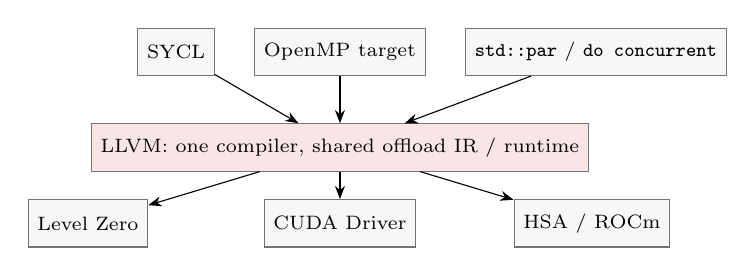
\begin{tikzpicture}[node distance=3.5mm and 5mm, >=Stealth, font=\scriptsize,
  b/.style={rectangle, draw=black!55, fill=black!3, minimum height=6mm, align=center},
  h/.style={rectangle, draw=black!55, fill=ANLRed!12, minimum height=6mm, align=center}]
  \node[b] (sycl) {SYCL};
  \node[b, right=of sycl] (omp) {OpenMP target};
  \node[b, right=of omp] (dc) {\texttt{std::par} / \texttt{do concurrent}};
  \node[h, below=6mm of omp] (llvm) {LLVM: one compiler, shared offload IR / runtime};
  \node[b, below=of llvm, xshift=-3.2cm] (l0)  {Level Zero};
  \node[b, below=of llvm]              (cu)  {CUDA Driver};
  \node[b, below=of llvm, xshift=3.2cm]  (hsa) {HSA / ROCm};
  \draw[->] (sycl)--(llvm); \draw[->] (omp)--(llvm); \draw[->] (dc)--(llvm);
  \draw[->] (llvm)--(l0); \draw[->] (llvm)--(cu); \draw[->] (llvm)--(hsa);
\end{tikzpicture}
\end{center}
\begin{itemize}
    \item SYCL is being \textbf{upstreamed into mainline LLVM} (Intel's \texttt{intel/llvm}
          tracks LLVM \texttt{main}, ~1--2 weeks behind).
    \item SYCL and OpenMP increasingly share the same LLVM offload plumbing\footnote{liboffload}  which route to the native backend: \textbf{Level~Zero}, \textbf{CUDA Driver}, \textbf{HSA}.
\end{itemize}

\end{frame}


\begin{frame}{Which one should I use?}
\begin{itemize}
    \item \textbf{Fortran?} $\rightarrow$ \textbf{OpenMP} (or \texttt{do concurrent}
          for standard-language offload). SYCL/Kokkos are C++-only.
    \item \textbf{C++, want close to the metal / an open standard?} $\rightarrow$
          \textbf{SYCL}. Lower-level, maps almost 1:1 to the native runtime.
    \item \textbf{C++, want data abstractions (\texttt{View}, layouts, \texttt{DualView})?}
          $\rightarrow$ \textbf{Kokkos}. Higher-level; sits on CUDA / HIP / SYCL.
          (Portability is a wash --- all three already cover the three vendors.)
    \item \textbf{Prototyping / data science / ML?} $\rightarrow$ \textbf{Python}
          (PyTorch, dpnp) --- same runtime underneath (SYCL on Intel, CUDA on
          NVIDIA; it does not reinvent either).
\end{itemize}
\alert{No wrong answer. Just use what you have support for.}
\end{frame}


\begin{frame}{Exp 2: benchmarks are always misleading}

\begin{itemize}
    \item I have 2 experiments. Watch, SYCL is the best!
    \item Let's see if we can flip the conclusion, the result
    \item Always take benchmarks with a grain of salt
\end{itemize}

\end{frame}


\begin{frame}{Conclusion}
    \begin{itemize}
        \item "same same, but different"
        \item If a gap exists, most probably it can be fixed in your code
        \item If not, it's probably a bug. Please report it
        \item My personal opinion:
            \begin{itemize}
                \item DON'T REINVENT ONE MORE
                \item Use the one where you have more support
            \end{itemize}
    \end{itemize}
\end{frame}

\begin{frame}{Last word}

The offload model is genuinely portable: between models and between vendors,
migration is cheap. The hard part is getting into the model. You must extract your compute kernels:
\begin{itemize}
    \item Isolate the kernel; hopefully an ``embarrassingly-parallel'' pure function
    \item Port the memory management

\end{itemize}
    
\end{frame}


% ATPESC acknowledgment / disclaimer -- text from ATPESC 2026 Template.pptx
\begin{frame}{Acknowledgments}
\footnotesize
\textbf{ARGONNE TRAINING PROGRAM ON EXTREME-SCALE COMPUTING}

\medskip
Produced by Argonne National Laboratory, a U.S. Department of Energy Laboratory
managed by UChicago Argonne, LLC under contract DE-AC02-06CH11357.

\medskip
Special thanks to the National Energy Research Scientific Computing Center
(NERSC) and Oak Ridge Leadership Computing Facility (OLCF) for the use of their
resources during the training event.

\medskip
The U.S. Government retains for itself and others acting on its behalf a
nonexclusive, royalty-free license in this video, with the rights to reproduce,
to prepare derivative works, and to display publicly.

\medskip
\texttt{extremecomputingtraining.anl.gov}
\end{frame}


\end{document}
